\chapter{A Mecânica dos Sólidos: tensão, deformação e deslocamento}

A Mecânica dos Sólidos é parte da física que estuda o comportamento de objetos sólidos sobre carregamentos, aplicando métodos analíticos para determinar suas características de resistência, rigidez e estabilidade. Seu conteúdo é notório por ser fundamental para grande parte da vida dos engenheiros, sendo mecânicos, civis ou mesmo eletricistas, ao lado de outras áreas também tão fundamentais, como Mecânica do Contínuo, Mecânica dos Fluidos e Termodinâmica. Sua aplicação é voltada ao projeto de estruturas a fim de que cumpram determinadas exigências, sejam tanto de deformação máxima, capacidade de carga e peso, como também de economia de materiais. E, por meio de ferramentas matemáticas, estuda os efeitos de tensão e deformação no interior de corpos sólidos. \cite{popov}

Este capítulo aborda os seguintes temas de Mecânica dos Sólidos, relevantes para o desenvolvimento inicial do módulo PHILLIPO.jl voltado à análise de estruturas elásticas sobre carregamentos contantes:
\begin{enumerate}
    \item tensão;
    \item deslocamento e deformação;
    \item a lei de Hooke generalizada;
    \item modelo de viga de Euler-Bernoulli;
    \item tensão de von mises.
\end{enumerate}

\section{Tensão}

Um corpo sólido se deforma quando submetido a carregamentos externos, distribuindo essas cargas ao longo de sua geometria. Tensão define a grandeza dessa distribuição agindo sobre áreas infinitesimais, de modo que qualquer secção do corpo revele forças internas que estejam em equilíbrio entre si, e que sejam balanceadas pelos carregamentos externos. Essas forças, geralmente, variam ao longo do corpo, como também, dependem do plano de seção. E, devido a sua forma vetorial, é conveniente que sejam decompostas em parcelas tangenciais e normais à seção. \cite{popov}

\begin{figure}
    \centering
    \caption{Forças internas: seção em um sólido qualquer}
    \begin{subfigure}[b]{\textwidth}
        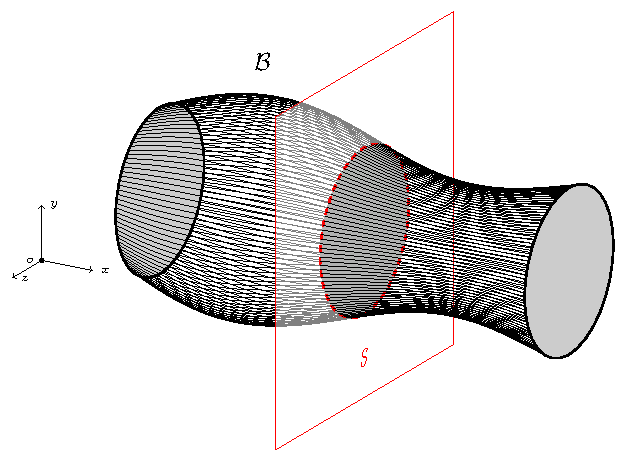
\includegraphics[scale=0.7]{Figuras/forcas_internas_2.pdf}
        \caption{$ $}
        \label{fig:forcas_internas_1}
    \end{subfigure}
    \hfill
    \begin{subfigure}[b]{\textwidth}
        \centering
        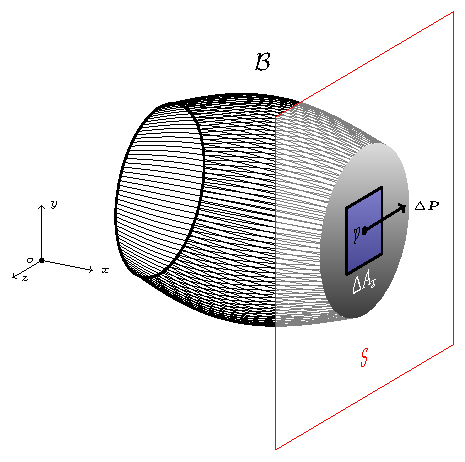
\includegraphics[scale=0.7]{Figuras/forcas_internas_1.pdf}
        \caption{$ $}
        \label{fig:forcas_internas_2}
    \end{subfigure}
    \hfill
    \begin{subfigure}[b]{\textwidth}
        \centering
        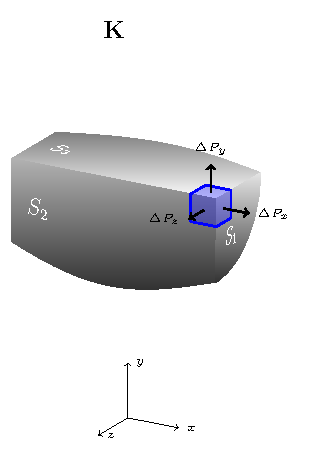
\includegraphics[scale=0.7]{Figuras/forcas_internas_3.pdf}
        \caption{$ $}
        \label{fig:forcas_internas_3}
    \end{subfigure}
       \label{fig:forcas_internas}
\end{figure}

Sejam um corpo $\bm{K}$, sólido, em equilíbrio e de geometria qualquer, submetido a forças externas na forma do carregamento $\vec{F}$, e as seções $S_{1,2,3}$, planos de corte através de esse corpo, ortogonais entre si, em que atuam as forças internas $\vec{P}$, conforme a figura \ref{fig:forcas_internas_1}. $\Delta P$ é a resultante de forças que atuam sobre uma área $\Delta A$ (centrada em um certo ponto $p$) discretizada de $S$. O limite da razão entre cada componente de $\Delta P$ (tangenciais e normais) e a área $\Delta A$, quando $\Delta A \to 0$, define a tensão sobre o ponto de análise do corpo. Em notação matemática tensão:

\begin{equation}
    \tau_{xx} = \lim_{\Delta A \to 0} \frac{\Delta P_x}{\Delta A}, \qquad
    \tau_{xy} = \lim_{\Delta A \to 0} \frac{\Delta P_y}{\Delta A}, \qquad
    \tau_{xz} = \lim_{\Delta A \to 0} \frac{\Delta P_z}{\Delta A},
\end{equation}
em que os índices de $\tau$ indicam, o primeiro, a normal do plano infinitesimal em que a tensão atua, e, o segundo, sua direção. Por conveniência, as tensões normais (aquelas que atuam perpendicularmente ao plano) são representadas por $\sigma$, ao invés de se utilizar $\tau$ com índices repetidos ($\tau_{xx} \equiv \sigma_x$). O símbolo $tau$, então, é reservado às tensões de cisalhamento, que atuam tangencialmente ao plano infinitesimal. No SI, a tensão é mensurada em Pascal [Pa](N/m²).

\begin{figure}
    \centering
    \caption{Estado de tensão}
    \begin{tikzpicture}[3d view = {-60}{-20}, scale=2]
        \draw[->] (0,0,0) --++ (3,0,0) node[right]{$x$};
        \draw[->] (0,0,0) --++ (0,3,0) node[left]{$y$};
        \draw[->] (0,0,0) --++ (0,0,3) node[above]{$z$};
        
        \draw[very thick, blue] (0,0,0) --++ (2,0,0) --++ (0,0,2)--++ (-2,0,0) -- cycle;
        \draw[very thick, blue] (0,2,0) --++ (2,0,0) --++ (0,0,2)--++ (-2,0,0) -- cycle;
        \draw[very thick, blue] (0,0,0) --++ (0,2,0) --++ (0,0,2) --++ (0,-2,0) -- cycle;
        \draw[very thick, blue] (2,0,0) --++ (0,2,0) --++ (0,0,2) --++ (0,-2,0) -- cycle;
        \draw[line width=1mm, blue, fill = blue, fill opacity = 0.5] (2,0,0) --++ (0,0,2) --++ (-2,0,0) --++ (0,2,0) --++ (0,0,-2) --+(2,0,0) -- cycle;
        
        
        \draw[arrows = {-Latex[width=10pt, length=10pt]},very thick, line width = 1mm] (2,1,1) --++ (1,0,0) node[right]{$\sigma_x$};
        \draw[arrows = {-Latex[width=10pt, length=10pt]},very thick, line width = 1mm] (1,2,1) --++ (0,1,0) node[left]{$\sigma_y$};
        \draw[arrows = {-Latex[width=10pt, length=10pt]},very thick, line width = 1mm] (1,1,2) --++ (0,0,1) node[right]{$\sigma_z$};
        
        \draw[arrows = {-Stealth[harpoon,swap]} ,very thick, line width = 1mm] (2,1,0.1) --++ (0,0,1.8) node[right]{$\tau_{xz}$};
        \draw[arrows = {-Stealth[harpoon]} ,very thick, line width = 1mm] (2,0.1,1) --++ (0,1.7,0) node[above]{$\tau_{xy}$};

        \draw[arrows = {-Stealth[harpoon]} ,very thick, line width = 1mm] (1,2,0.1) --++ (0,0,1.8) node[left]{$\tau_{yz}$};
        \draw[arrows = {-Stealth[harpoon,swap]} ,very thick, line width = 1mm] (0.1,2,1) --++ (1.7,0,0) node[below]{$\tau_{yx}$};               
        
        \draw[arrows = {-Stealth[harpoon]} ,very thick, line width = 1mm] (0.1,1,2) --++ (1.8,0,0) node[left]{$\tau_{zx}$};
        \draw[arrows = {-Stealth[harpoon,swap]} ,very thick, line width = 1mm] (1,0.1,2) --++ (0,1.8,0) node[above]{$\tau_{zy}$};        
        
        
    \end{tikzpicture}
    \label{fig:estado_de_tensao}
\end{figure}

Se o mesmo procedimento for realizado para cada face de um elemento cúbico, formado por mais três seções paralelas e equidistantes a $S_{1,2,3}$ da figura \ref{fig:forcas_internas_3}, teremos a configuração da tensão em três planos perpendiculares entre si para um certo ponto $p$ em $\bm{K}$,  conforme a figura \ref{fig:estado_de_tensao}, o que descreve o estado de tensão para aquele ponto. É conveniente escrever as componentes do estado de tensão na forma

\begin{equation}
    [\sigma] =
    \begin{bmatrix}
        \sigma_x & \tau_{xy} & \tau_{xz} \\
        \tau_{yx} & \sigma_{y} & \tau_{yz} \\
        \tau_{zx} & \tau_{zy} & \sigma_{z} \\
    \end{bmatrix},
\end{equation}
em que a linha indica o plano em que a componente age, e a coluna, sua direção.

!!!continua...!!!

\section{Deslocamento e deformação}

O deslocamento de um sólido por ser descrito por uma função vetorial que mapeia cada ponto do domínio ao seu respectivo deslocamento, de modo que é igual à variação ente a posição original e a deslocada do ponto.

Seja um corpo $\bm{K}$ definido sobre uma região $\Omega$, e a função $\vec{U}(\vec{x})$, a representação de seu deslocamento, que descreve a transformação da posição original em deformada de cada ponto, mapeando $\Omega$ para $\Omega'$.

\begin{equation}
    T(\vec{x}) = \vec{x} \vec{x} + \vec{U}(\vec{x}),
    \vec{U}_{\bm{K}}(x,y,z) = \begin{bmatrix}
        u(x,y,z) \\ v(x,y,z) \\ w(x,y,z) 
    \end{bmatrix}.
\end{equation}
em que $u, v, w$ são as componentes do deslocamento nas direções de $x, y, z$, respectivamente.

\begin{figure}
    \centering
    \caption{Função de deslocamento sobre a região de um sólido}
    \begin{tikzpicture}[
        mdomain/.style = {blue, line width = 0.5mm, fill = blue, fill opacity = 0.3},
        marrow/.style={arrows = {-Stealth[length=8pt, inset=5pt]}, line width = 0.2mm},
        marrowb/.style={arrows = {-Stealth[length=10pt, inset=1pt]}, line width = 0.5mm, violet},
        marrowc/.style={arrows = {-Stealth[length=10pt, inset=3pt]}, line width = 0.5mm}
        ]
    ]
        \draw[mdomain] plot[smooth, variable=\u, domain=0:360]({(5 * cos(\u) + 0.3 * sin(\u))/1.5 + 3.5},{(2 * sin(\u) + 0.4 * cos(3 *\u))/1.5+5});
        \draw[mdomain] plot[smooth, variable=\u, domain=0:360, blue, thick, fill = blue, fill opacity = 0.6]({(5 * cos(\u) + 0.3 * sin(\u))/2 +10},{(2 * sin(\u) + 0.4 * cos(3 *\u))/1.1+3});

        \node[white, scale = 4, opacity = 0.5] (Ca) at (3.5,5) {\large $\Omega$};

        \node[white, scale = 4, opacity = 0.5] (Cb) at (10,3) {\large $\Omega'$};

        \draw[->] (0,0) -- (12,0) node[above]{$x$};
        \draw[->] (0,0) -- (0,6) node[above]{$y$};

        \node[] (A) at (4,4) {};
        \draw (A) node[above right]{$A$};
        \node[] (B) at (3,6) {};
        \draw (B) node[above]{$B$};

        \node[] (A') at (8,2.8) {};
        \draw (A') node[above]{$A'$};
        \node (B') at (11.5,3) {};
        \draw (B') node[above right]{$B'$};
        
        \draw[magenta, line width = 0.5mm] (A.center) -- (B.center);
        \draw[magenta, line width = 0.5mm] (A'.center) -- (B'.center);

        \draw[marrow]  (0,0) -- (A.center) node[midway,above left]{\large $\vec{a}$};
        \draw[marrow]  (0,0) -- (B.center) node[midway,above left]{\large $\vec{b}$};
        \draw[marrow]  (0,0) -- (A'.center) node[midway,above]{\large $\vec{a}'$};
        \draw[marrow]  (0,0) -- (B'.center) node[midway,below]{\large $\vec{b}'$};

        \draw[marrowb]  (A.center) -- (A'.center) node[midway,below]{$\vec{U}(\vec{A})$};
        \draw[marrowb]  (B.center) -- (B'.center) node[midway,below]{$\vec{U}(\vec{B})$};

        \foreach \n in {A,B,A',B'}
             \node at (\n)[circle,fill,inner sep=0.3mm]{};

        \draw[marrowc] (6.4,6) to[out=45, in=125] (9, 5.2); 
        
        \node[scale = 2] (T) at (8.5,6.6) {$T$};

    \end{tikzpicture}
    \label{fig:deslocamento}
\end{figure}

\section{A Lei de Hooke}

Em corpos sólidos, a deformação está relacionada diretamente com a tensão em seu interior, de modo que se possa, dentro de certas condições, descrever uma transformação linear entre elas. Essa transformação é nomeada \emph{Lei de Hooke}.

Sejam a barra $\bm{B}$, um corpo sólido, homogêneo, em equilíbrio, de comprimento $L$, engastado em $x=0$, e de seção transversal quadrada $A$, e $F$, uma força constante que atua sobre a face direita de $\bm{B}$, na direção de $x$, que a deforma em $\bm{B}'$ até um comprimento $L+\Delta L$, tal como na figura \ref{fig:barra_deformada}. 

\begin{figure}
    \centering
    \caption{Barra deformada}
    \begin{subfigure}[b]{\textwidth}
        \resizebox{\textwidth}{!}{
            \begin{tikzpicture}[
                    marrow/.style = {arrows = {-Latex[width=8pt, length=10pt]}}
                ]
                
                \draw[->] (0,0) --++ (0,3) node[above]{$y$};
                \draw[->] (0,0) --++ (10,0) node[above]{$x$};

                \draw[thick, blue, fill = blue, fill opacity = 0.3] (0,0) rectangle (8,2);
                \draw (4,1) node{$\bm{B}$};
                
                \draw[thick, blue, fill = blue, fill opacity = 0.3, dashed] (0,0.2) rectangle (8.5,1.8);

                \draw[|<->|] (0,2.1) --++ (8,0) node[above, midway]{$L$};
                \draw[|<->|] (8,2.1) --++ (0.5,0) node[above,midway]{$\Delta L$};

                \draw[marrow] (8.5,1) --++ (2,0) node[right]{$\vec{F}$};
                
            \end{tikzpicture}
        }
        \caption{por tração}
        \label{fig:barra_deformada_1}
    \end{subfigure}
    \begin{subfigure}[b]{\textwidth}
        \resizebox{\textwidth}{!}{
            \begin{tikzpicture}[
                marrow/.style = {arrows = {-Latex[width=4pt, length=10pt]}, line width = 0.5mm}
            ]

            \draw[->] (0,0) --++ (0,3) node[above]{$y$};
            \draw[->] (0,0) --++ (10,0) node[above]{$x$};
            \draw[thick] (8,2)-- (8,3.10) (8,0) -- (8.5,2) --++ (0.25, 1);
            \draw[thick, blue, fill = blue, fill opacity = 0.3, dashed] (0,0) rectangle (8,2);


            \draw[thick, red, fill = red, fill opacity = 0.3] (0,0) -- (0.5,2) -- (8.5,2) -- (8,0) -- cycle;

            \draw[|<->|] (0,2.1) --++ (8,0) node[above, midway]{$L$};
            \foreach \n in {0,1,...,7}{
                \draw[marrow] ({\n},2) --++ (1.05,0);
            }

            \draw (1,2) |- (2,3) node[right]{$Q$};
            \draw (4,1) node{$\bm{B}$};

            \draw[<->] (8,2.7) arc (90:71:2) node[midway, above]{$\gamma$}	;
            \end{tikzpicture}
        }
        \caption{por cisalhamento}
        \label{fig:barra_deformada_2}
    \end{subfigure}
\end{figure}

A tensão desenvolvida em uma seção $S$ de $\bm{B}$, perpendicular à força $\vec{F}$, pode ser descrita em termos do módulo de elasticidade do material que compõe $\bm{B}$, $E$ (denominado também de Módulo de ), e da deformação $\Delta L$, de modo que

\begin{equation}
    \sigma_x = E \epsilon_x = E \frac{\Delta L}{L}.
\end{equation}